\documentclass[12pt]{article}
\usepackage[utf8]{inputenc}
\usepackage[a4paper, margin=2cm]{geometry}
\usepackage[T1]{fontenc}
\usepackage{graphicx}
\usepackage{geometry}
\usepackage{amsmath}
\usepackage{amsfonts}
\usepackage{amssymb}
\usepackage{booktabs}
\usepackage{hyperref}
\usepackage{fancyhdr}
\usepackage{float}
\usepackage{ulem}
\usepackage{xeCJK}
\usepackage{listings}
\usepackage{xcolor}
\usepackage{indentfirst}
\setmainfont{Times New Roman}
\setCJKmonofont[BoldFont=SimHei, AutoFakeBold=true]{SimSun}
\lstset{
    basicstyle=\ttfamily\small,
    commentstyle=\color{gray},
    keywordstyle=\color{blue},
    stringstyle=\color{red},
    numberstyle=\tiny\color{gray},
    breaklines=true,
    captionpos=b,
    keepspaces=true,
    numbers=left,
    numbersep=5pt,
    showspaces=false,
    showstringspaces=false,
    showtabs=false,
    tabsize=2,
    frame=single,
    language=[x86masm]Assembler
}

\begin{document}
\thispagestyle{empty}

\begin{center}
    \vspace*{2cm}
    
    \Huge \textbf{2023-2024学年春季学期} \\
    \vspace{2cm}
    
    \Huge \textbf{《汇编语言程序设计》} \\
    \vspace{4cm}
    
    \large 评分：\underline{\hspace{4cm}} \\
    \vspace{6cm}
    
    \begin{tabular}{rl}
        \Large 学\hspace{2em}院： & \Large \underline{\makebox[12em][l]{\quad 计算机科学与工程学院}} \\
        \Large 专\hspace{2em}业： & \Large \underline{\makebox[12em][l]{\quad 计算机科学与技术}} \\
        \Large 班\hspace{2em}级： & \Large \underline{\makebox[12em][l]{\quad 计算机2204班}} \\
        \Large 姓\hspace{2em}名： & \Large \underline{\makebox[12em][l]{\quad 李俊洁}} \\
        \Large 学\hspace{2em}号： & \Large \underline{\makebox[12em][l]{\quad 20225443}} \\
        \Large 任课教师：         & \Large \underline{\makebox[12em][l]{\quad 刘思宇、柳秀梅}} \\
    \end{tabular}
    \vfill
\end{center}
\newpage

\section{实验目的}
本实验的主要目的是通过编程练习，深入了解和掌握x86汇编语言，特别是关于条件跳转和系统调用的使用。
此外，实验也旨在加强对程序控制流程的理解和应用。具体目标包括：
\begin{itemize}
    \item 掌握如何在汇编语言中处理带符号的整数数据，并进行条件判断。
    \item 学习使用系统调用来实现屏幕上的字符输出。
    \item 了解如何在程序中使用条件跳转指令来实现复杂的逻辑判断。
    \item 增强使用DEBUG工具进行程序调试的技能，特别是在输入和输出数据验证方面。
    \item 培养分析和解决问题的能力，通过实验修正和优化代码。
\end{itemize}

这次实验也将加强我的代码调试技能，帮助我更好地理解和解决程序中可能遇到的问题。
这部分内容确保我们能通过具体的编程任务来实际应用理论知识。
\section{实验要求}
本实验要求学生通过具体的编程任务，深入理解x86汇编语言的基本构造和控制流程，特别是在进行逻辑判断和屏幕输出操作时的细节。
实验的要求如下：
\begin{itemize}
    \item 使用x86汇编语言编写要求的程序，并且能够实现屏幕的字符输出。
    \item 分别用三组数据（同时为正，同时为负，异号）调试程序，验证程序的正确性。第一组数据在源程序中给出，第二组和第三组数据要求在DEBUG下用E命令给出。
    \item 编写清晰的代码注释，解释每个主要步骤的功能和目的，以便日后的代码维护或复查。
    \item 在实验报告中详细记录每次实验的输入数据和输出结果，包括使用DEBUG修改数据的步骤和屏幕截图。
    \item 绘制程序的流程图，以清楚展示程序逻辑和各个步骤的连接，有助于更好地理解程序结构。
\end{itemize}

\section{实验内容}
已知DATA单元开始存放三个带符号数，编制程序，检查三个数据是否同号，若同时为正，则在显示器上显示“+”；
同时为负，则显示“-”；否则显示空格“\;”。

分别用三组数据（同时为正，同时为负，异号）调试程序，验证程序的正确性。
第一组数据在源程序中给出，第二组和第三组数据要求在DEBUG下用E命令给出。

\section{源程序}
    \begin{lstlisting}[caption={汇编源代码}, label=lst:asm2]
dseg    segment
data    db 1, 1, 1
; data    db -1, -1, -1
; data    db 0, 1, -1
dseg    ends

sseg    segment  stack
stack   db  100h  dup  (?)
sseg    ends

cseg    segment
    assume cs:cseg, ds:dseg, ss:sseg

start:
    ; 初始化
    mov ax, dseg
    mov ds, ax
    mov ax, sseg
    mov ss, ax
    mov sp, 100h
    xor ax, ax
    xor bx, bx
    xor cx, cx

    ; 加载第一个数据
    mov al, data
    cmp al, 1
    jge positive
    cmp al, -1
    jle negative
    jmp show_blank

positive:
    ; 第一个数据为正
    mov bl, data + 1
    cmp bl, 0
    jle show_blank
    ; 第二个数据为正
    mov cl, data + 2
    cmp cl, 0
    jle show_blank
    ; 第三个数据为正
    jmp show_positive

negative:
    ; 第一个数据为负
    mov bl, data + 1
    cmp bl, 0
    jge show_blank
    ; 第二个数据为负
    mov cl, data + 2
    cmp cl, 0
    jge show_blank
    ; 第三个数据为负
    jmp show_negative

show_blank:
    ; 显示空白
    mov dl, ' '
    mov ah, 02h
    int 21h
    jmp return

show_positive:
    ; 显示正号
    mov dl, '+'
    mov ah, 02h
    int 21h
    jmp return

show_negative:
    ; 显示负号
    mov dl, '-'
    mov ah, 02h
    int 21h

return:
    ; 结束程序
    mov ah, 4ch
    int 21h

cseg    ends
    end start
    \end{lstlisting}

\section{运行结果}
    \subsection{显示结果}
    三种数据时分别的显示结果：

    全正，显示加号：
    \begin{center}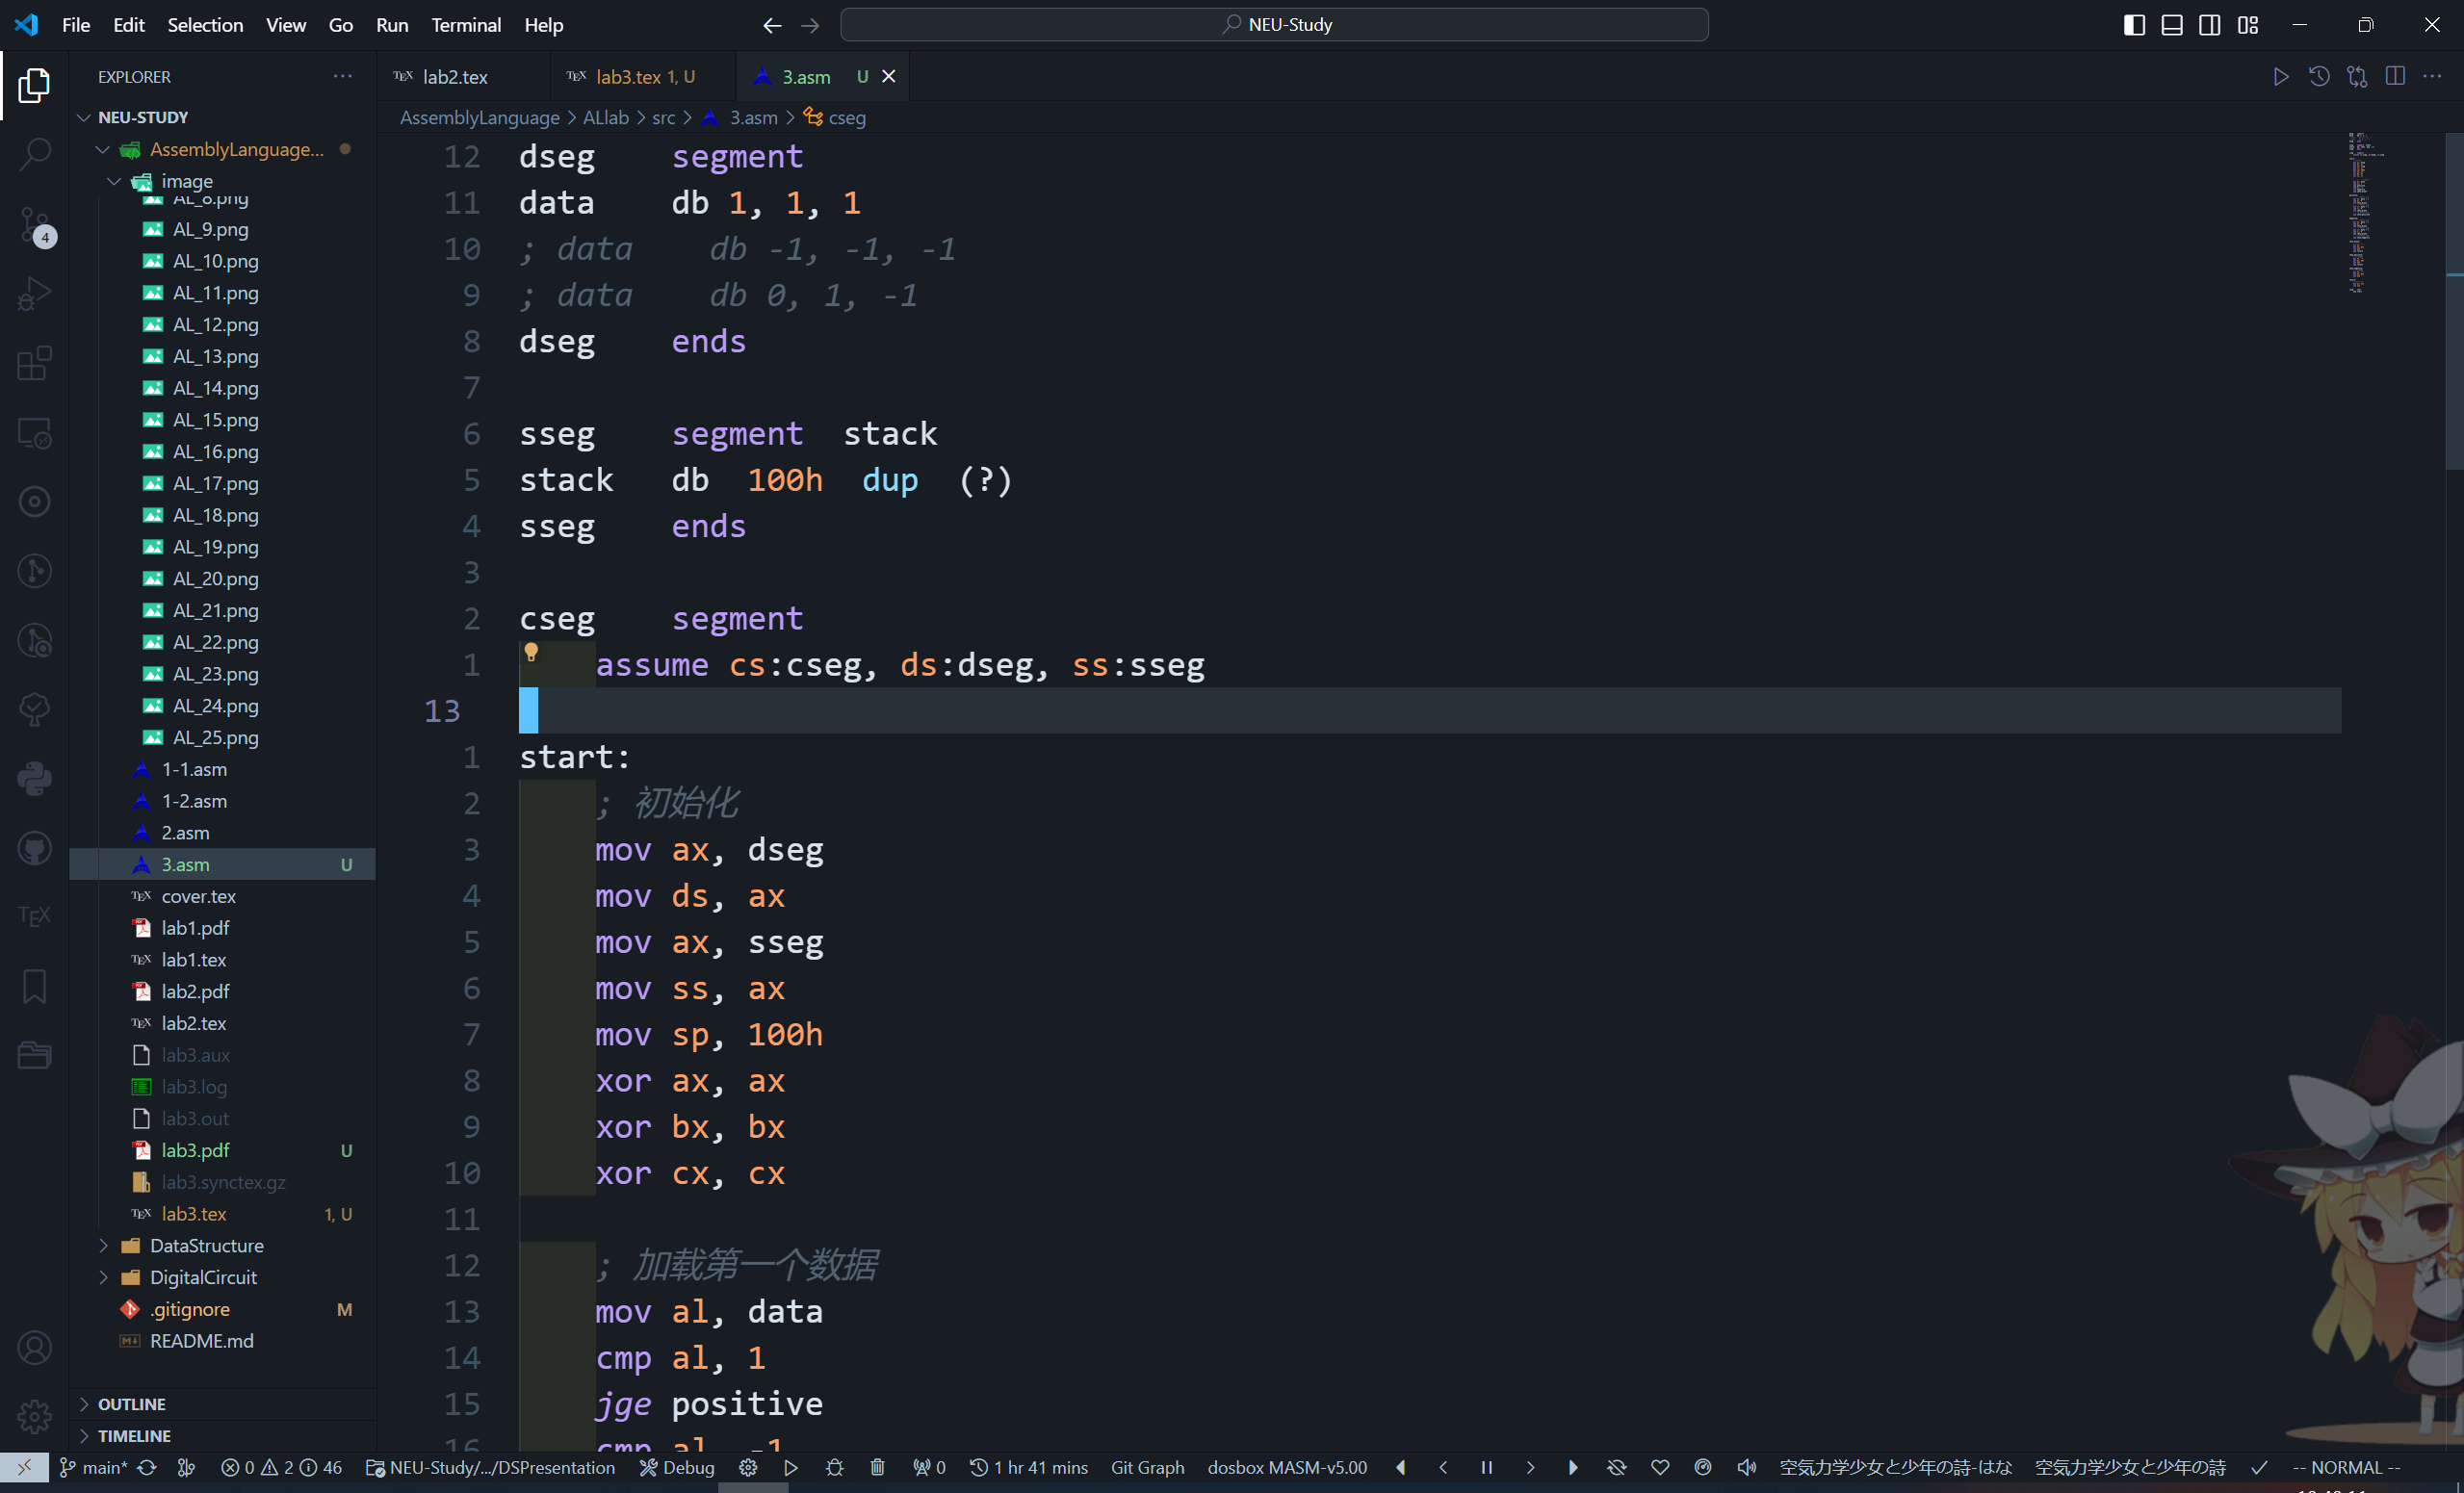
\includegraphics[width=1\textwidth]{image/AL_26.png}\end{center}
    \begin{center}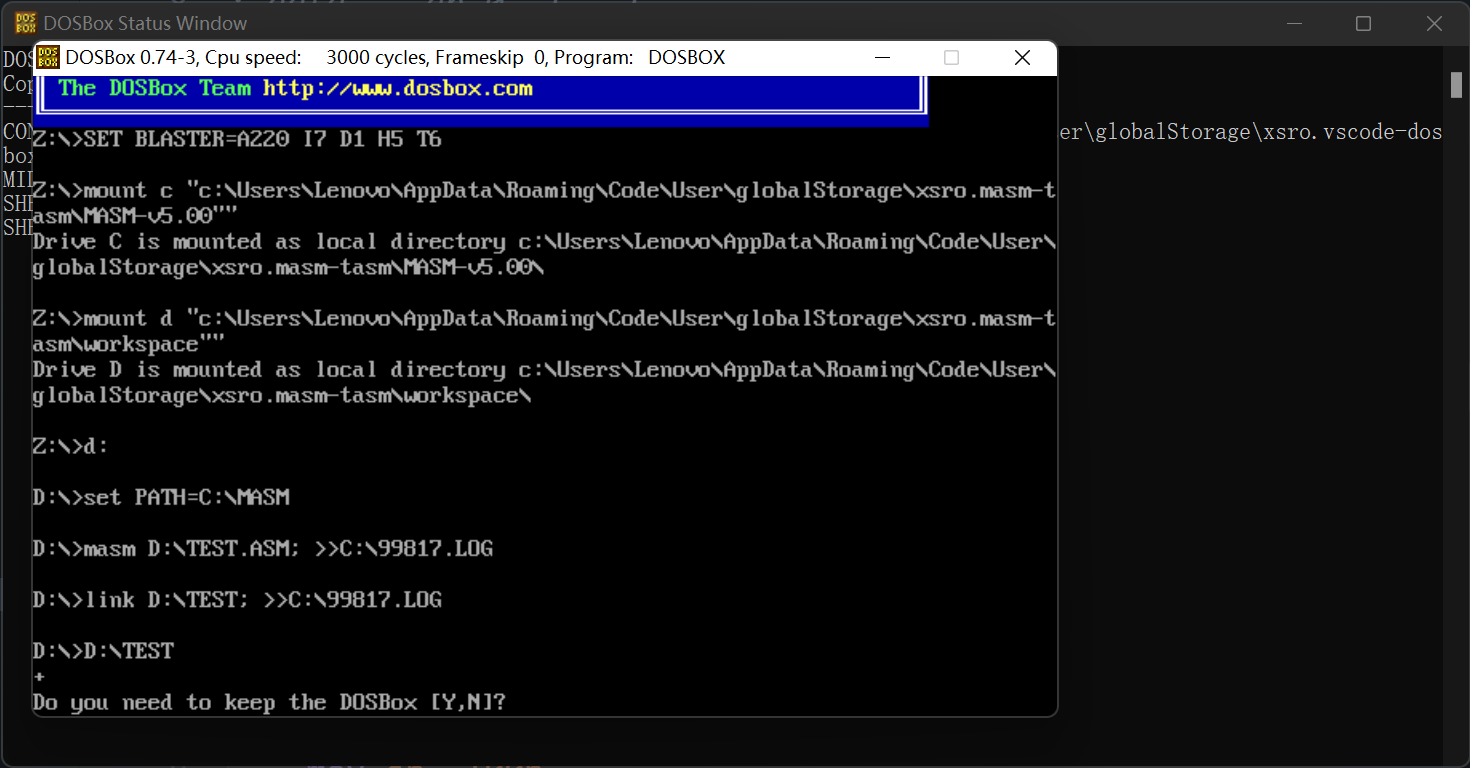
\includegraphics[width=1\textwidth]{image/AL_27.png}\end{center}
    全负，显示符号：
    \begin{center}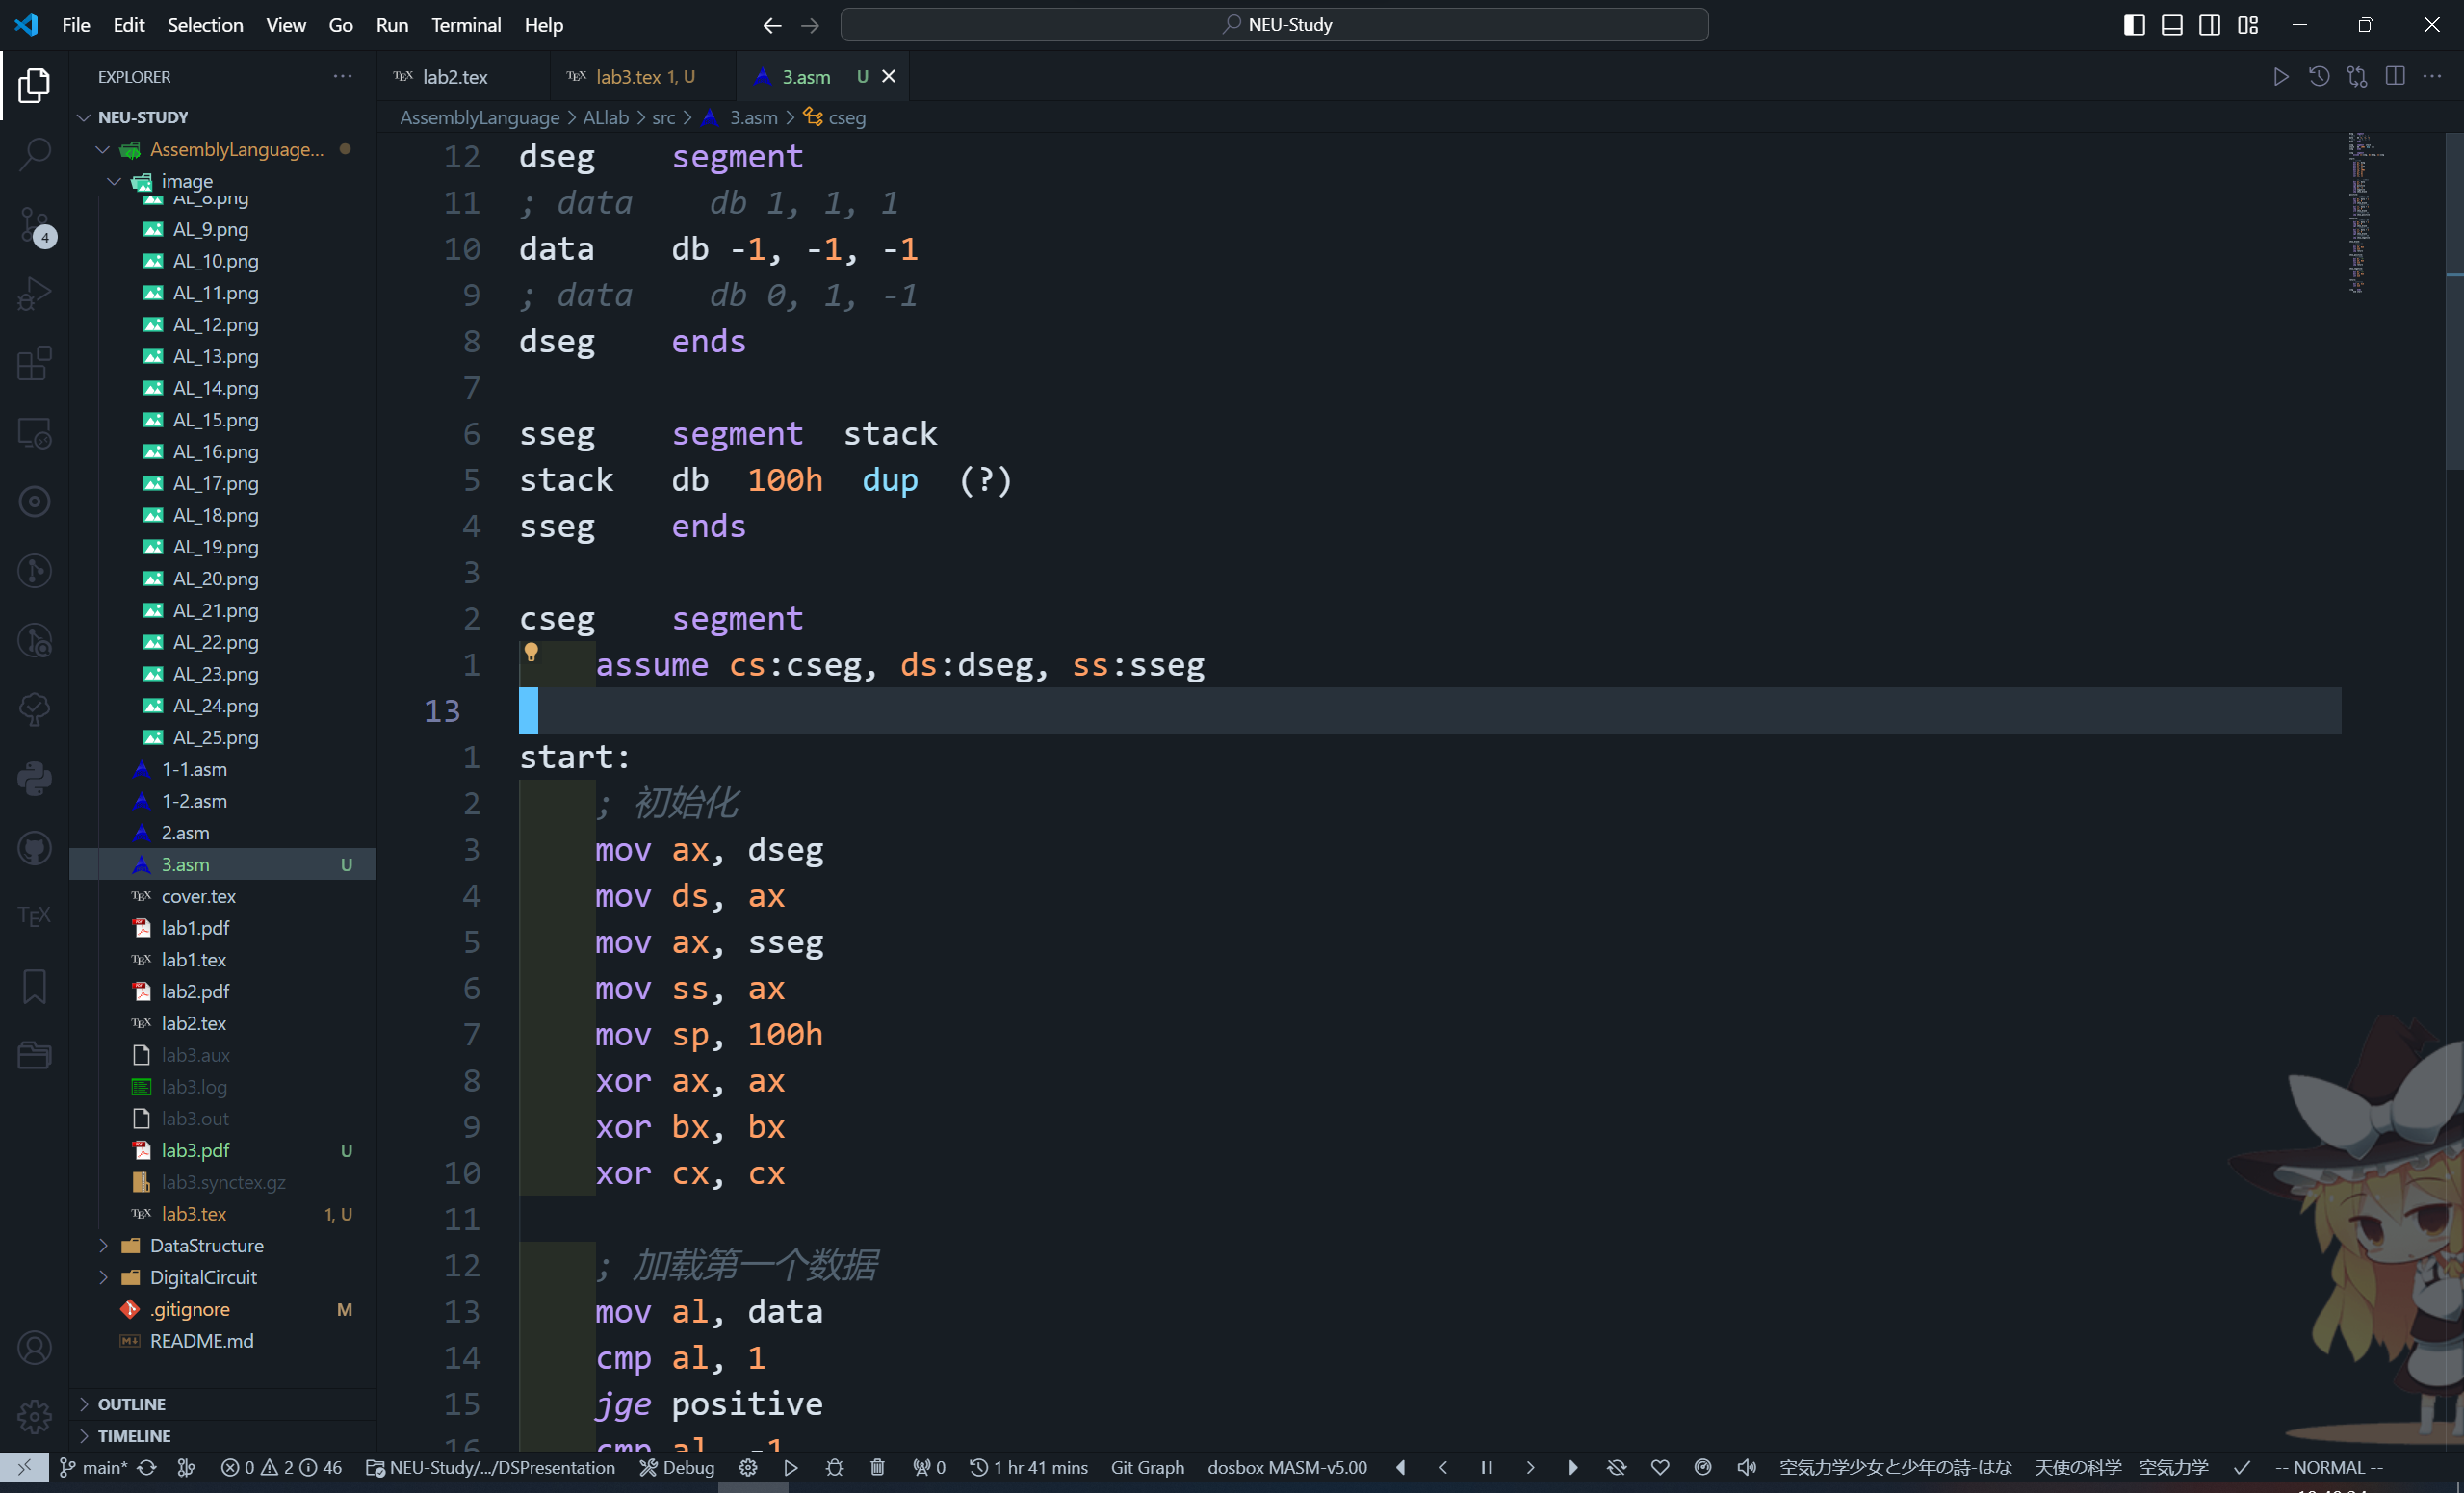
\includegraphics[width=1\textwidth]{image/AL_28.png}\end{center}
    \begin{center}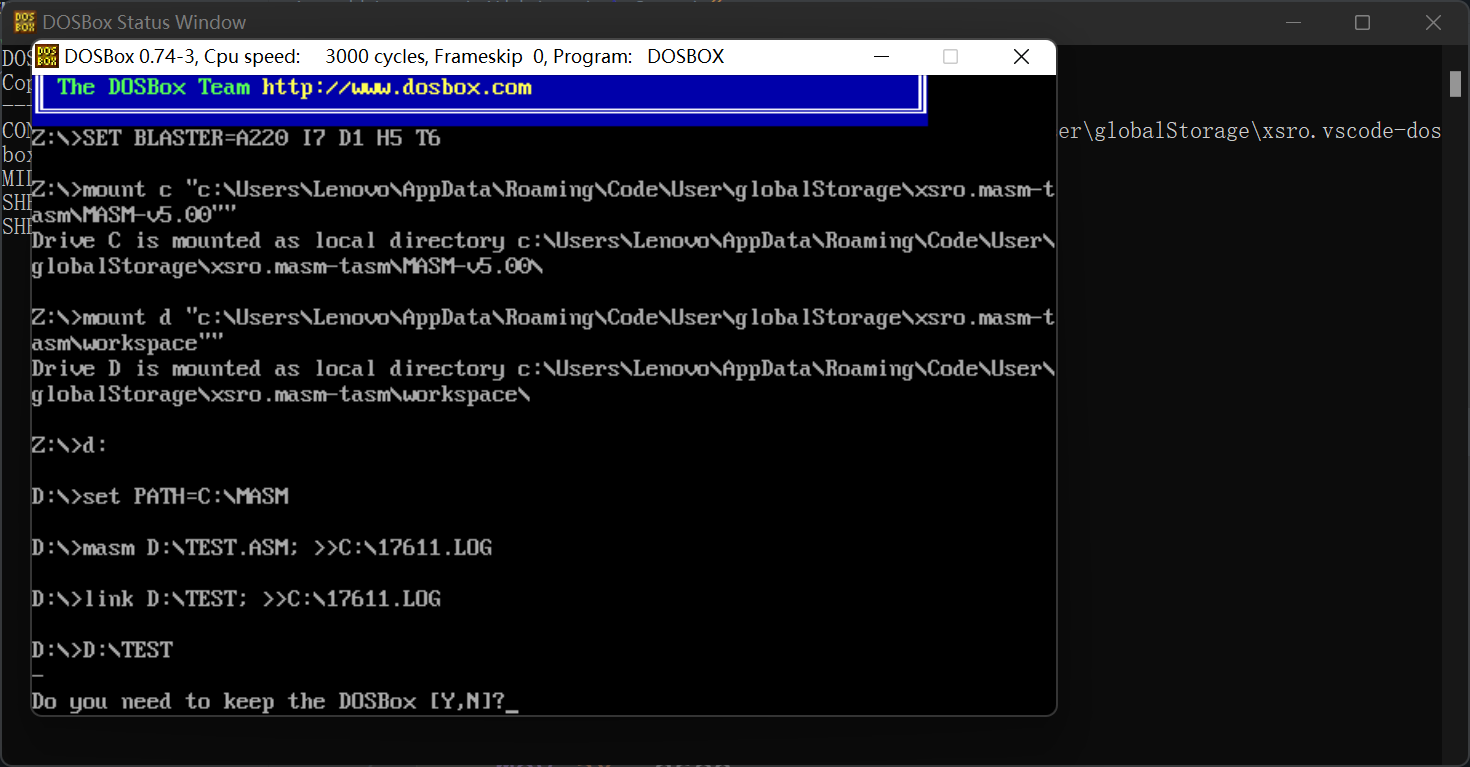
\includegraphics[width=1\textwidth]{image/AL_29.png}\end{center}
    混乱的情况，显示空格：
    \begin{center}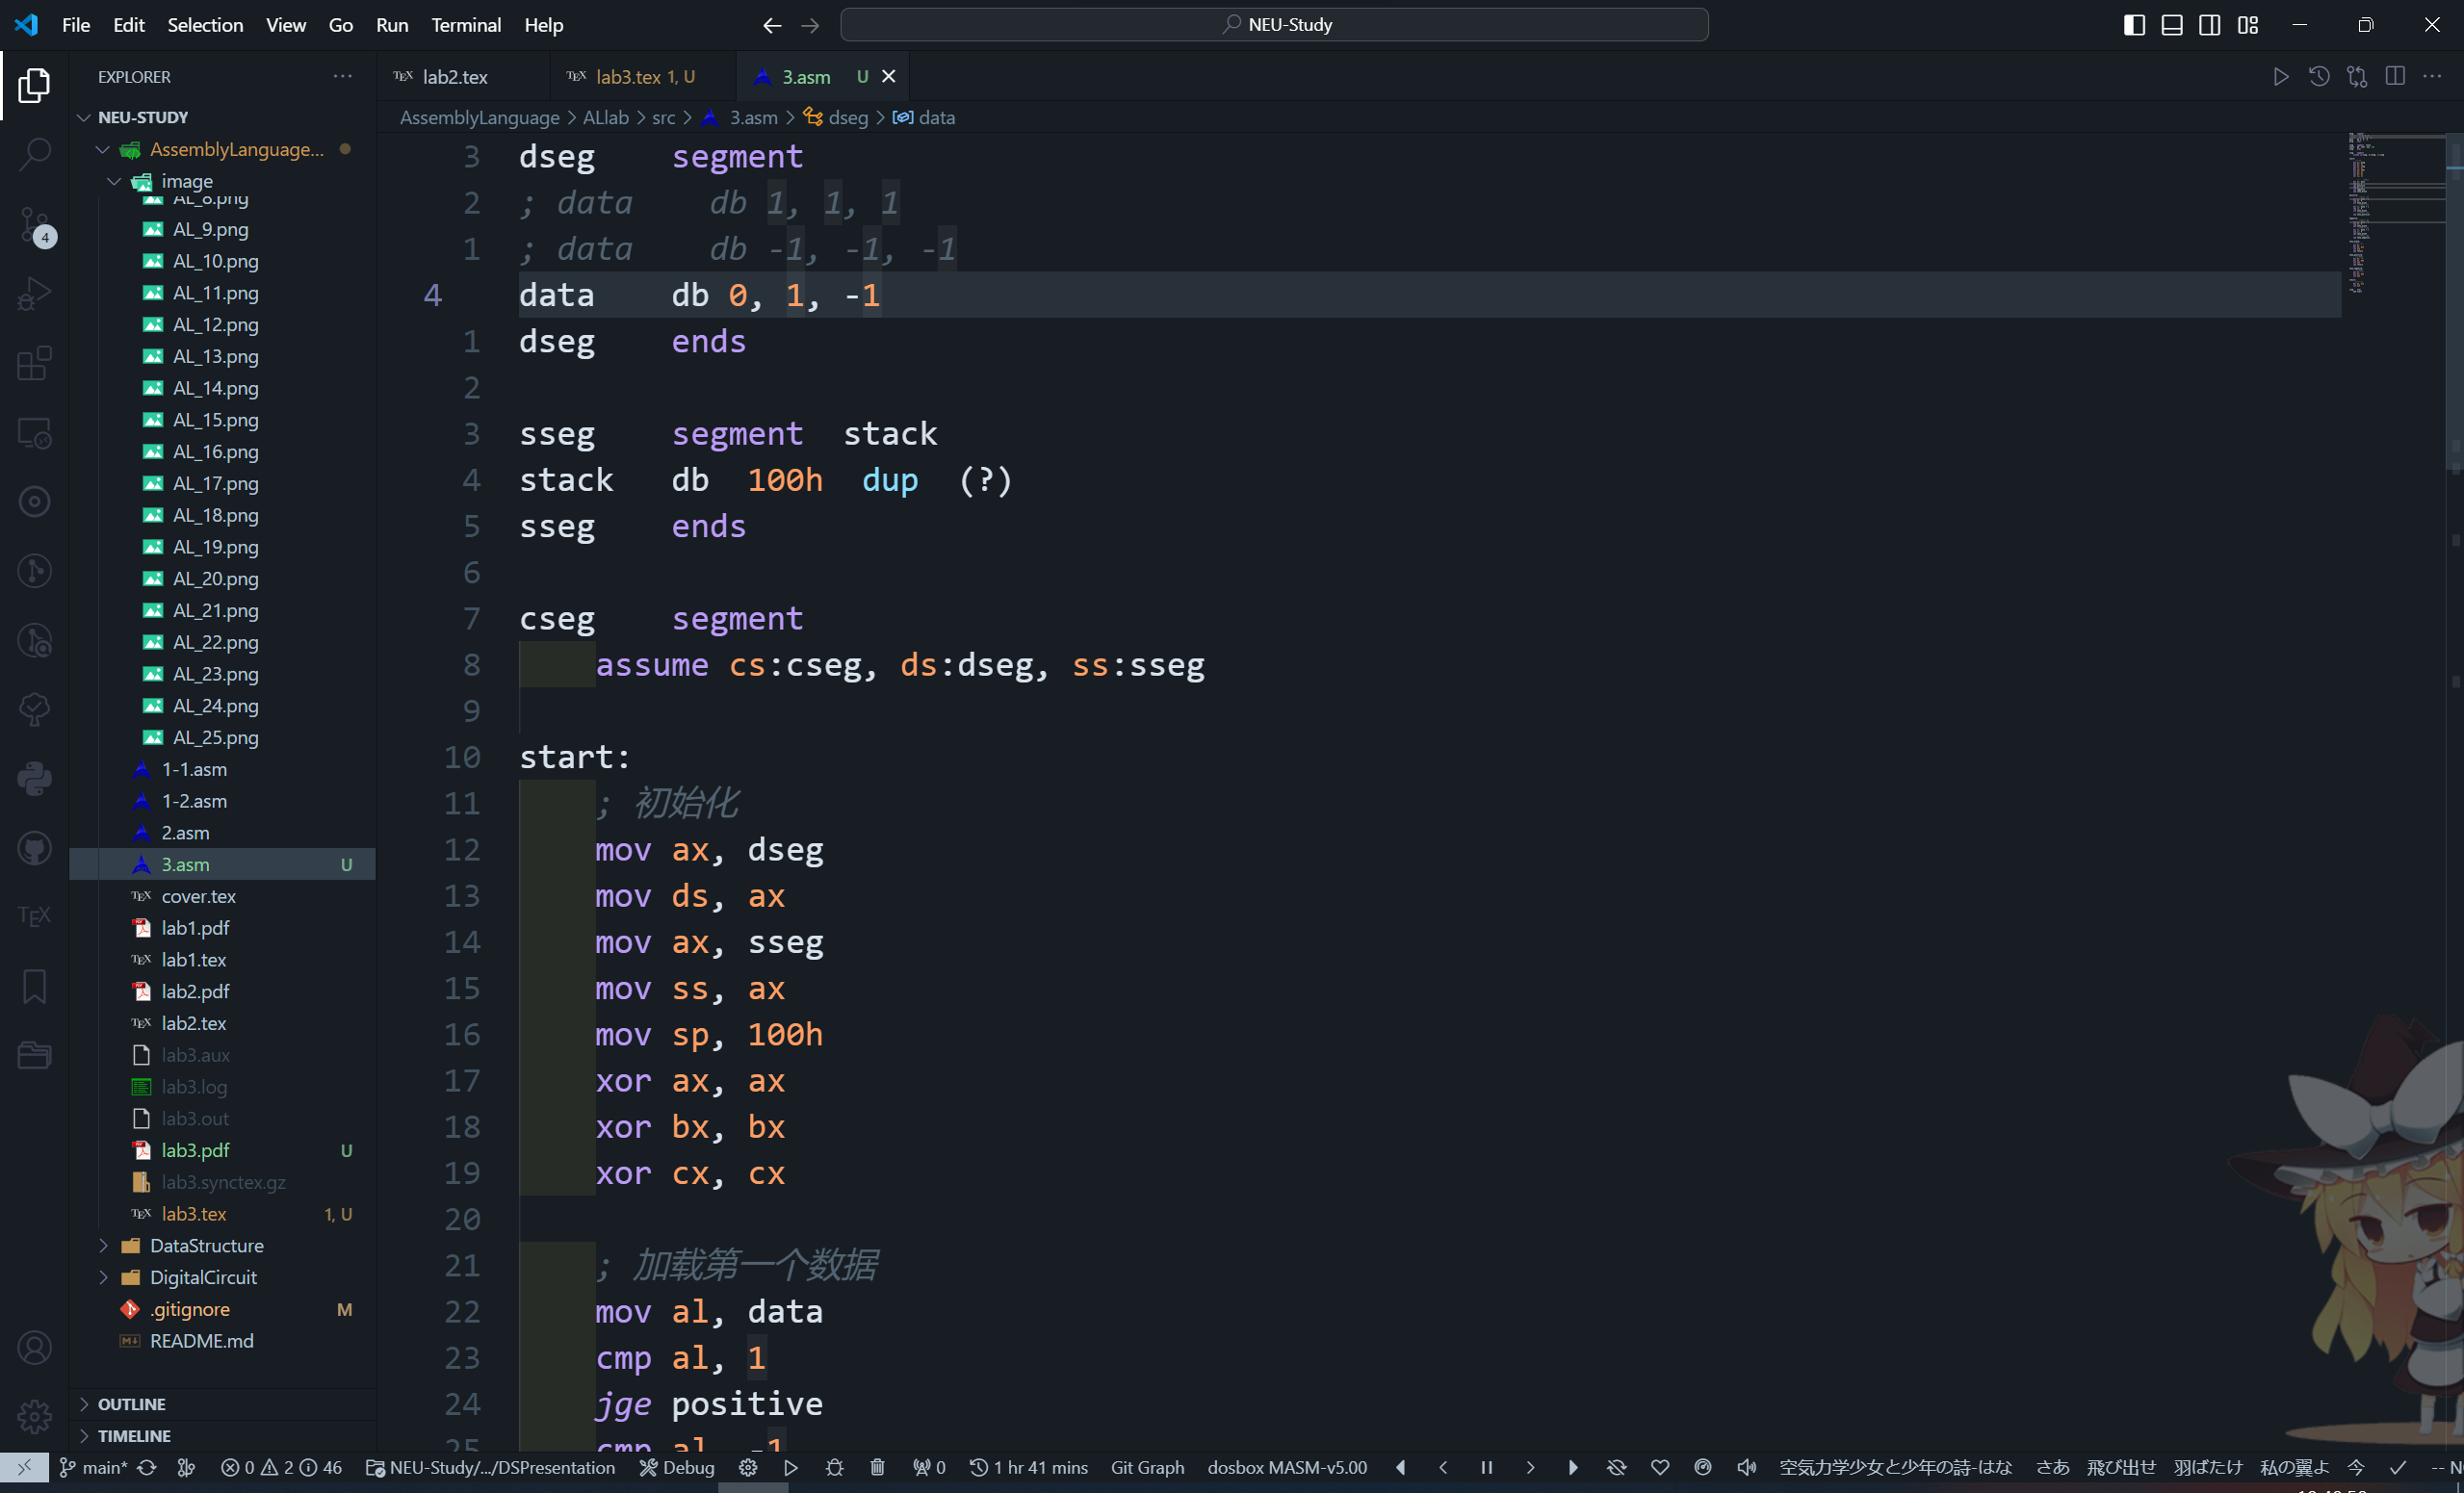
\includegraphics[width=1\textwidth]{image/AL_30.png}\end{center}
    \begin{center}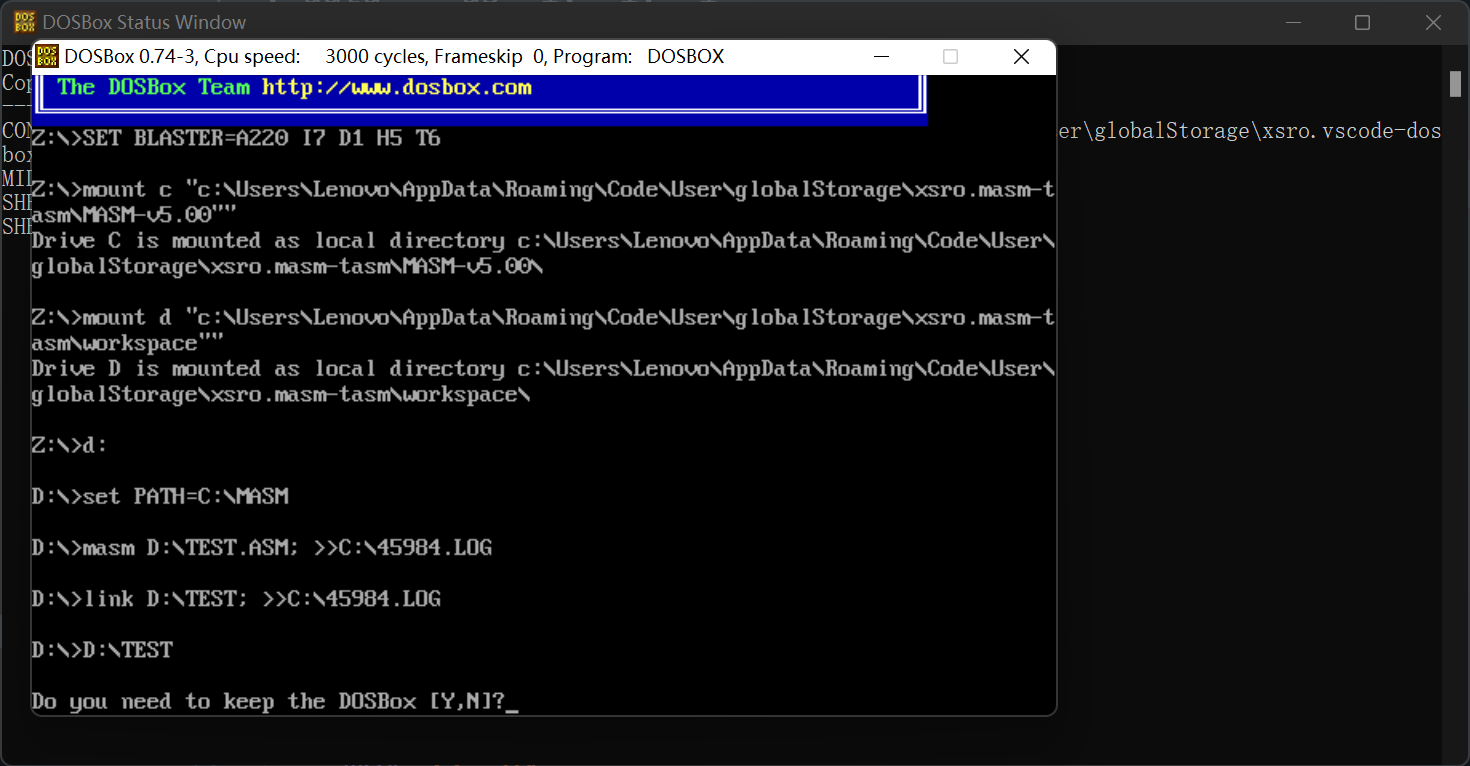
\includegraphics[width=1\textwidth]{image/AL_31.png}\end{center}
    \subsection{调试步骤}
    本来输出的是空格：
    \begin{center}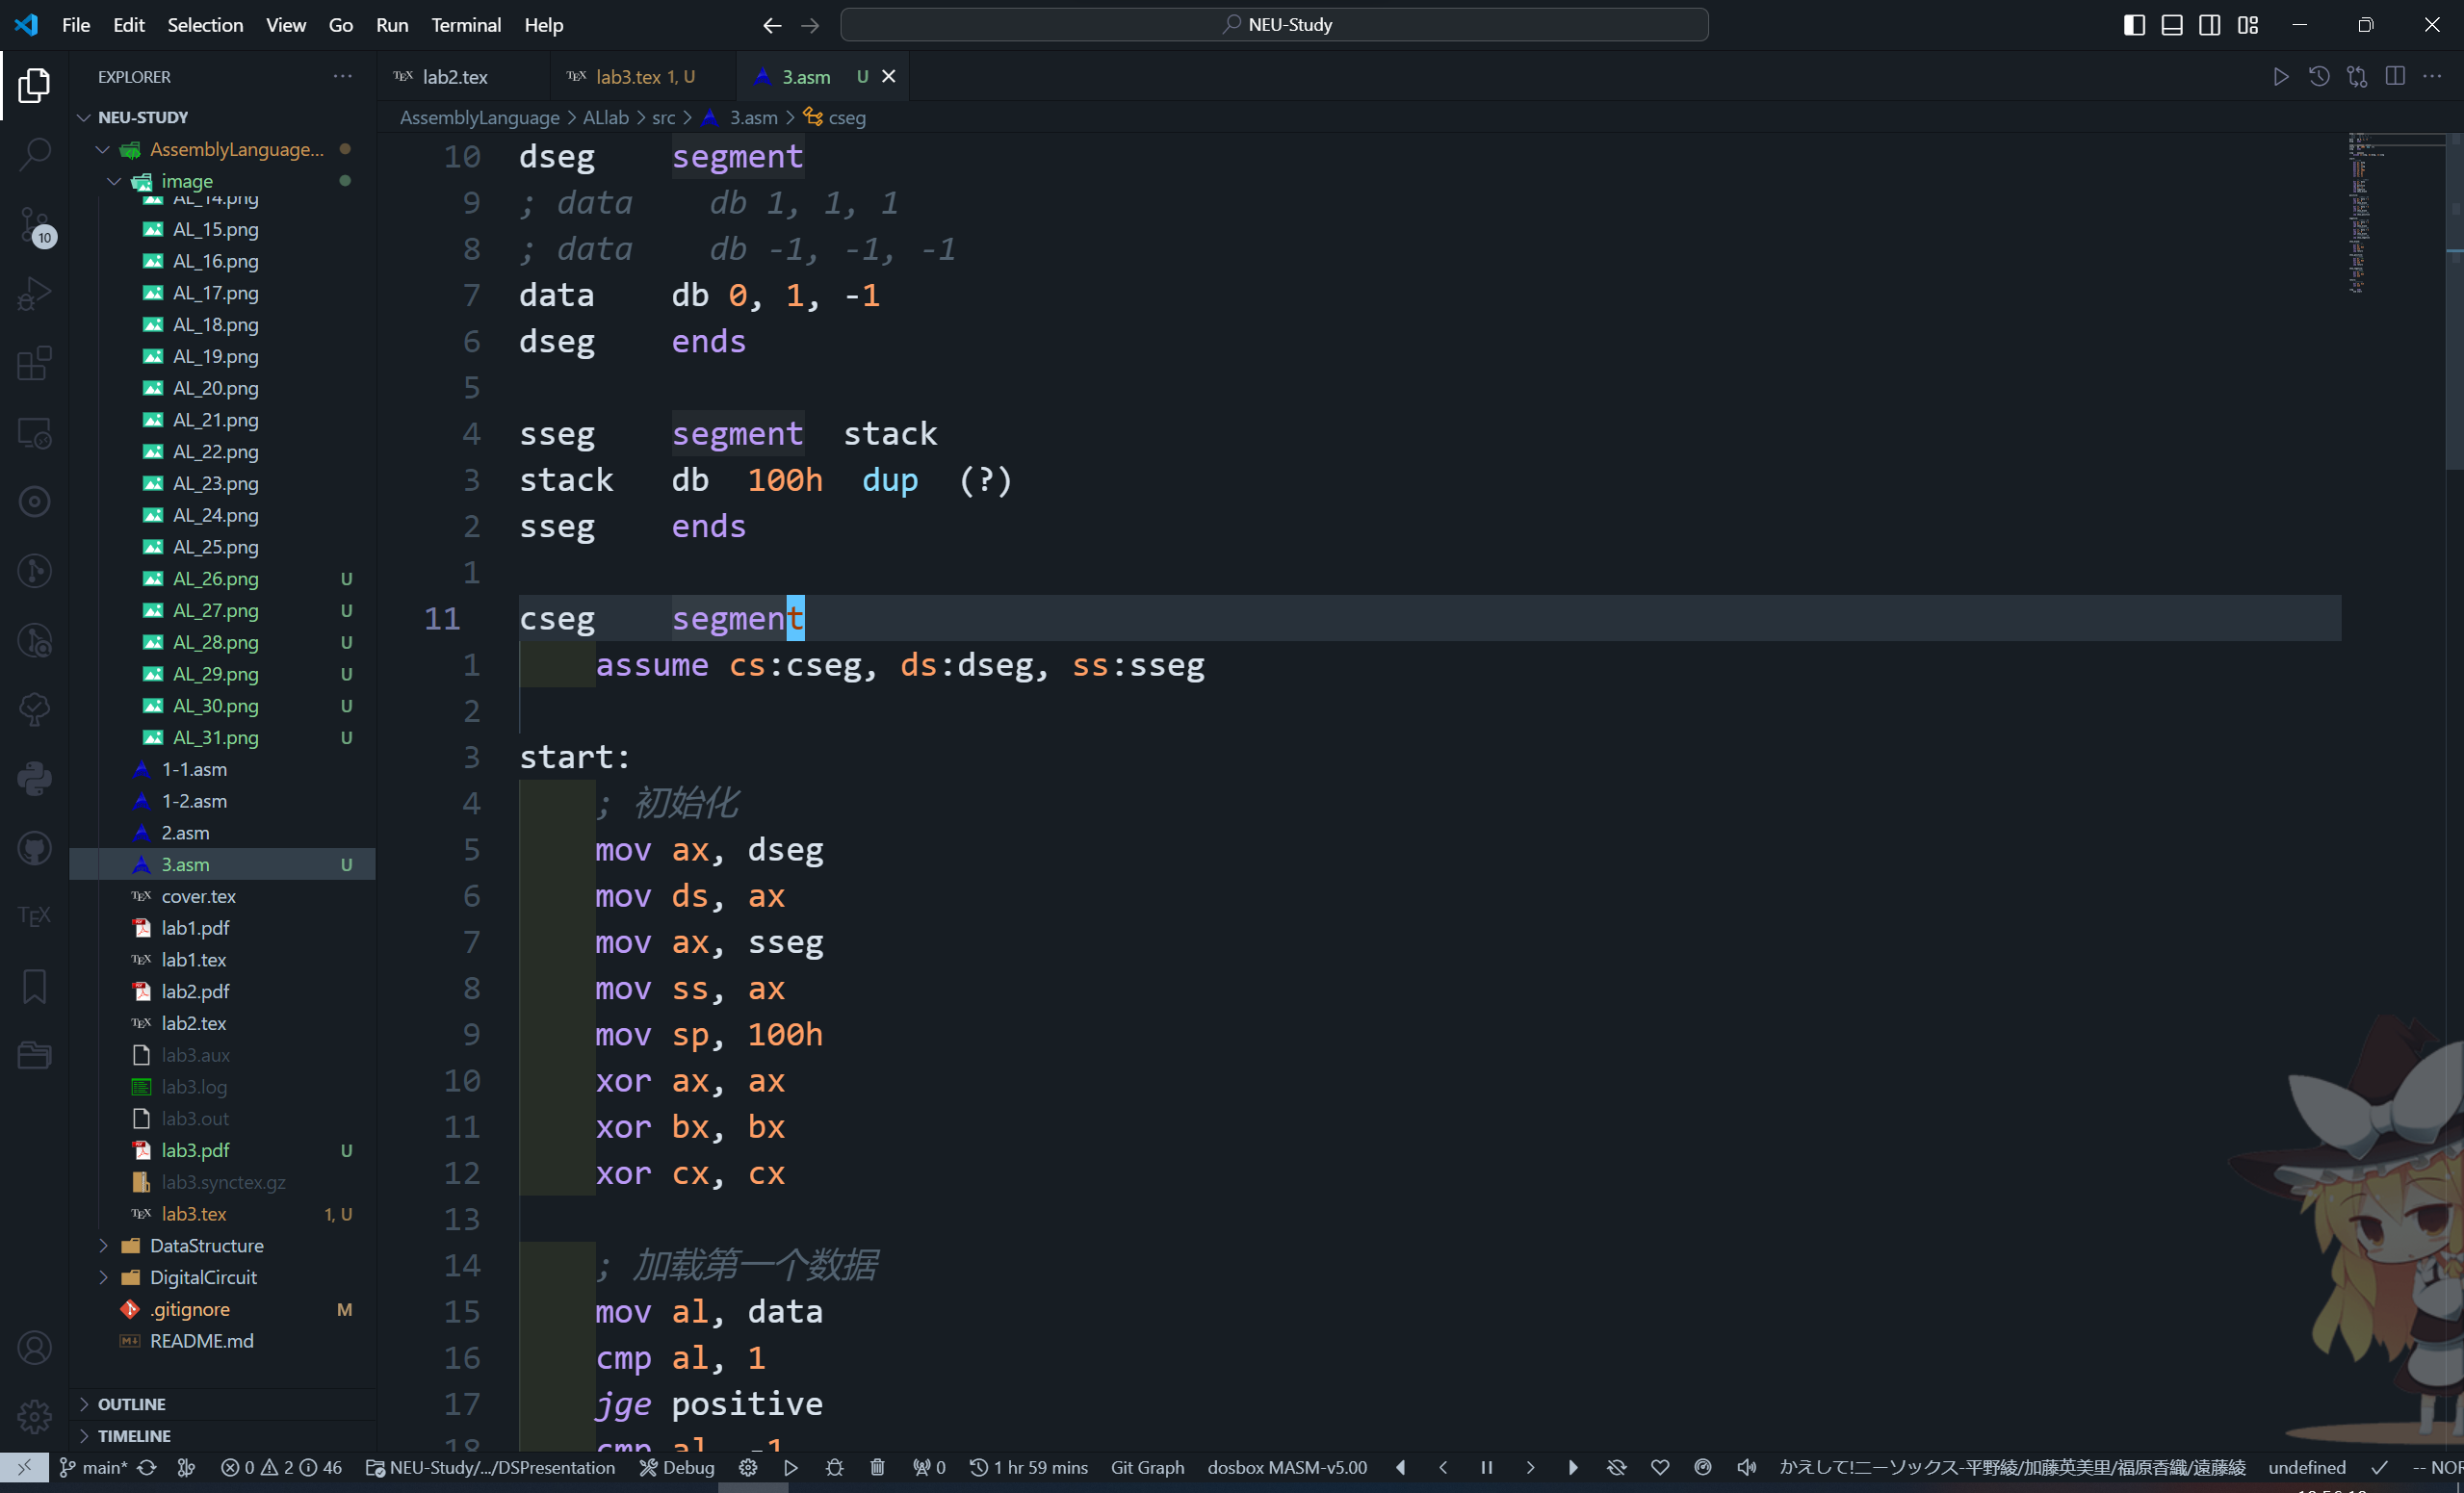
\includegraphics[width=1\textwidth]{image/AL_32.png}\end{center}
    修改数据为正数：
    \begin{center}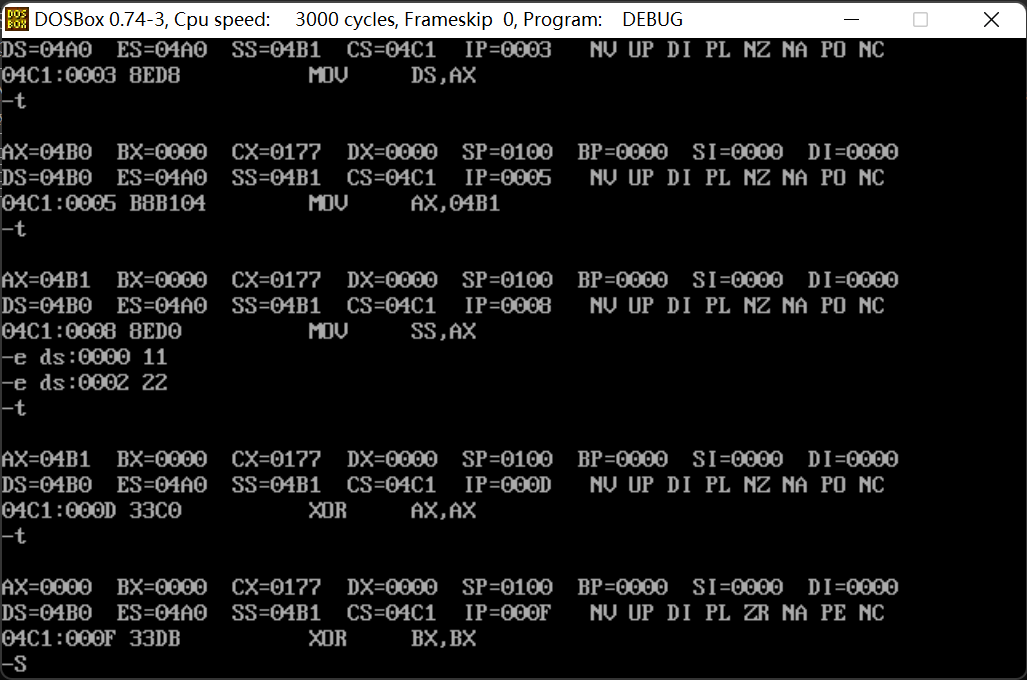
\includegraphics[width=1\textwidth]{image/AL_33.png}\end{center}
    输出加号：
    \begin{center}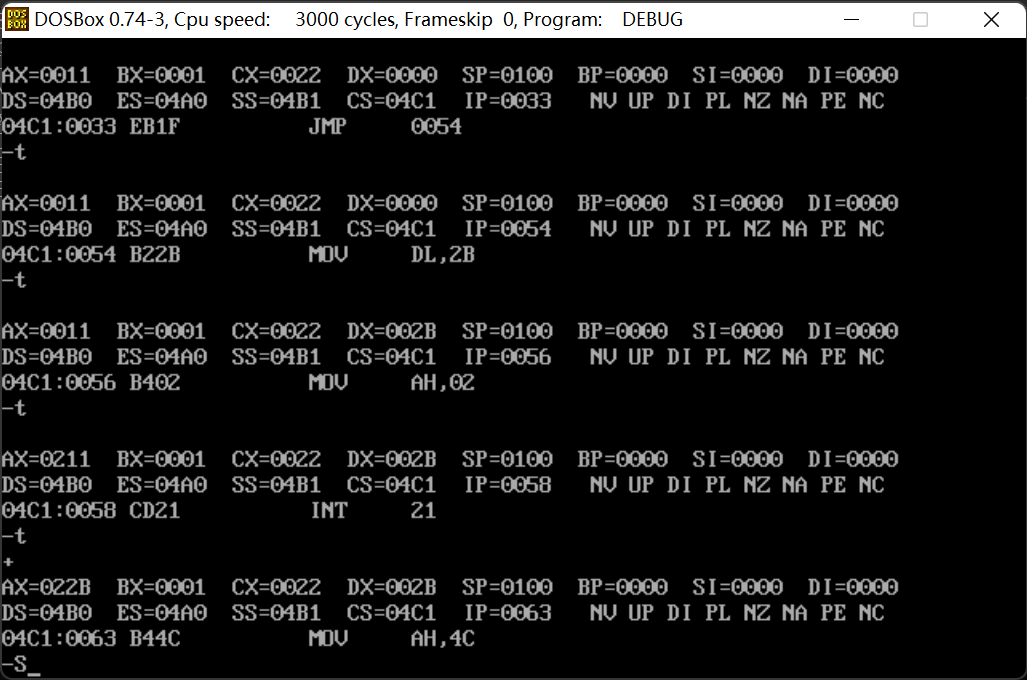
\includegraphics[width=1\textwidth]{image/AL_34.png}\end{center}
    本来输出的是加号：
    \begin{center}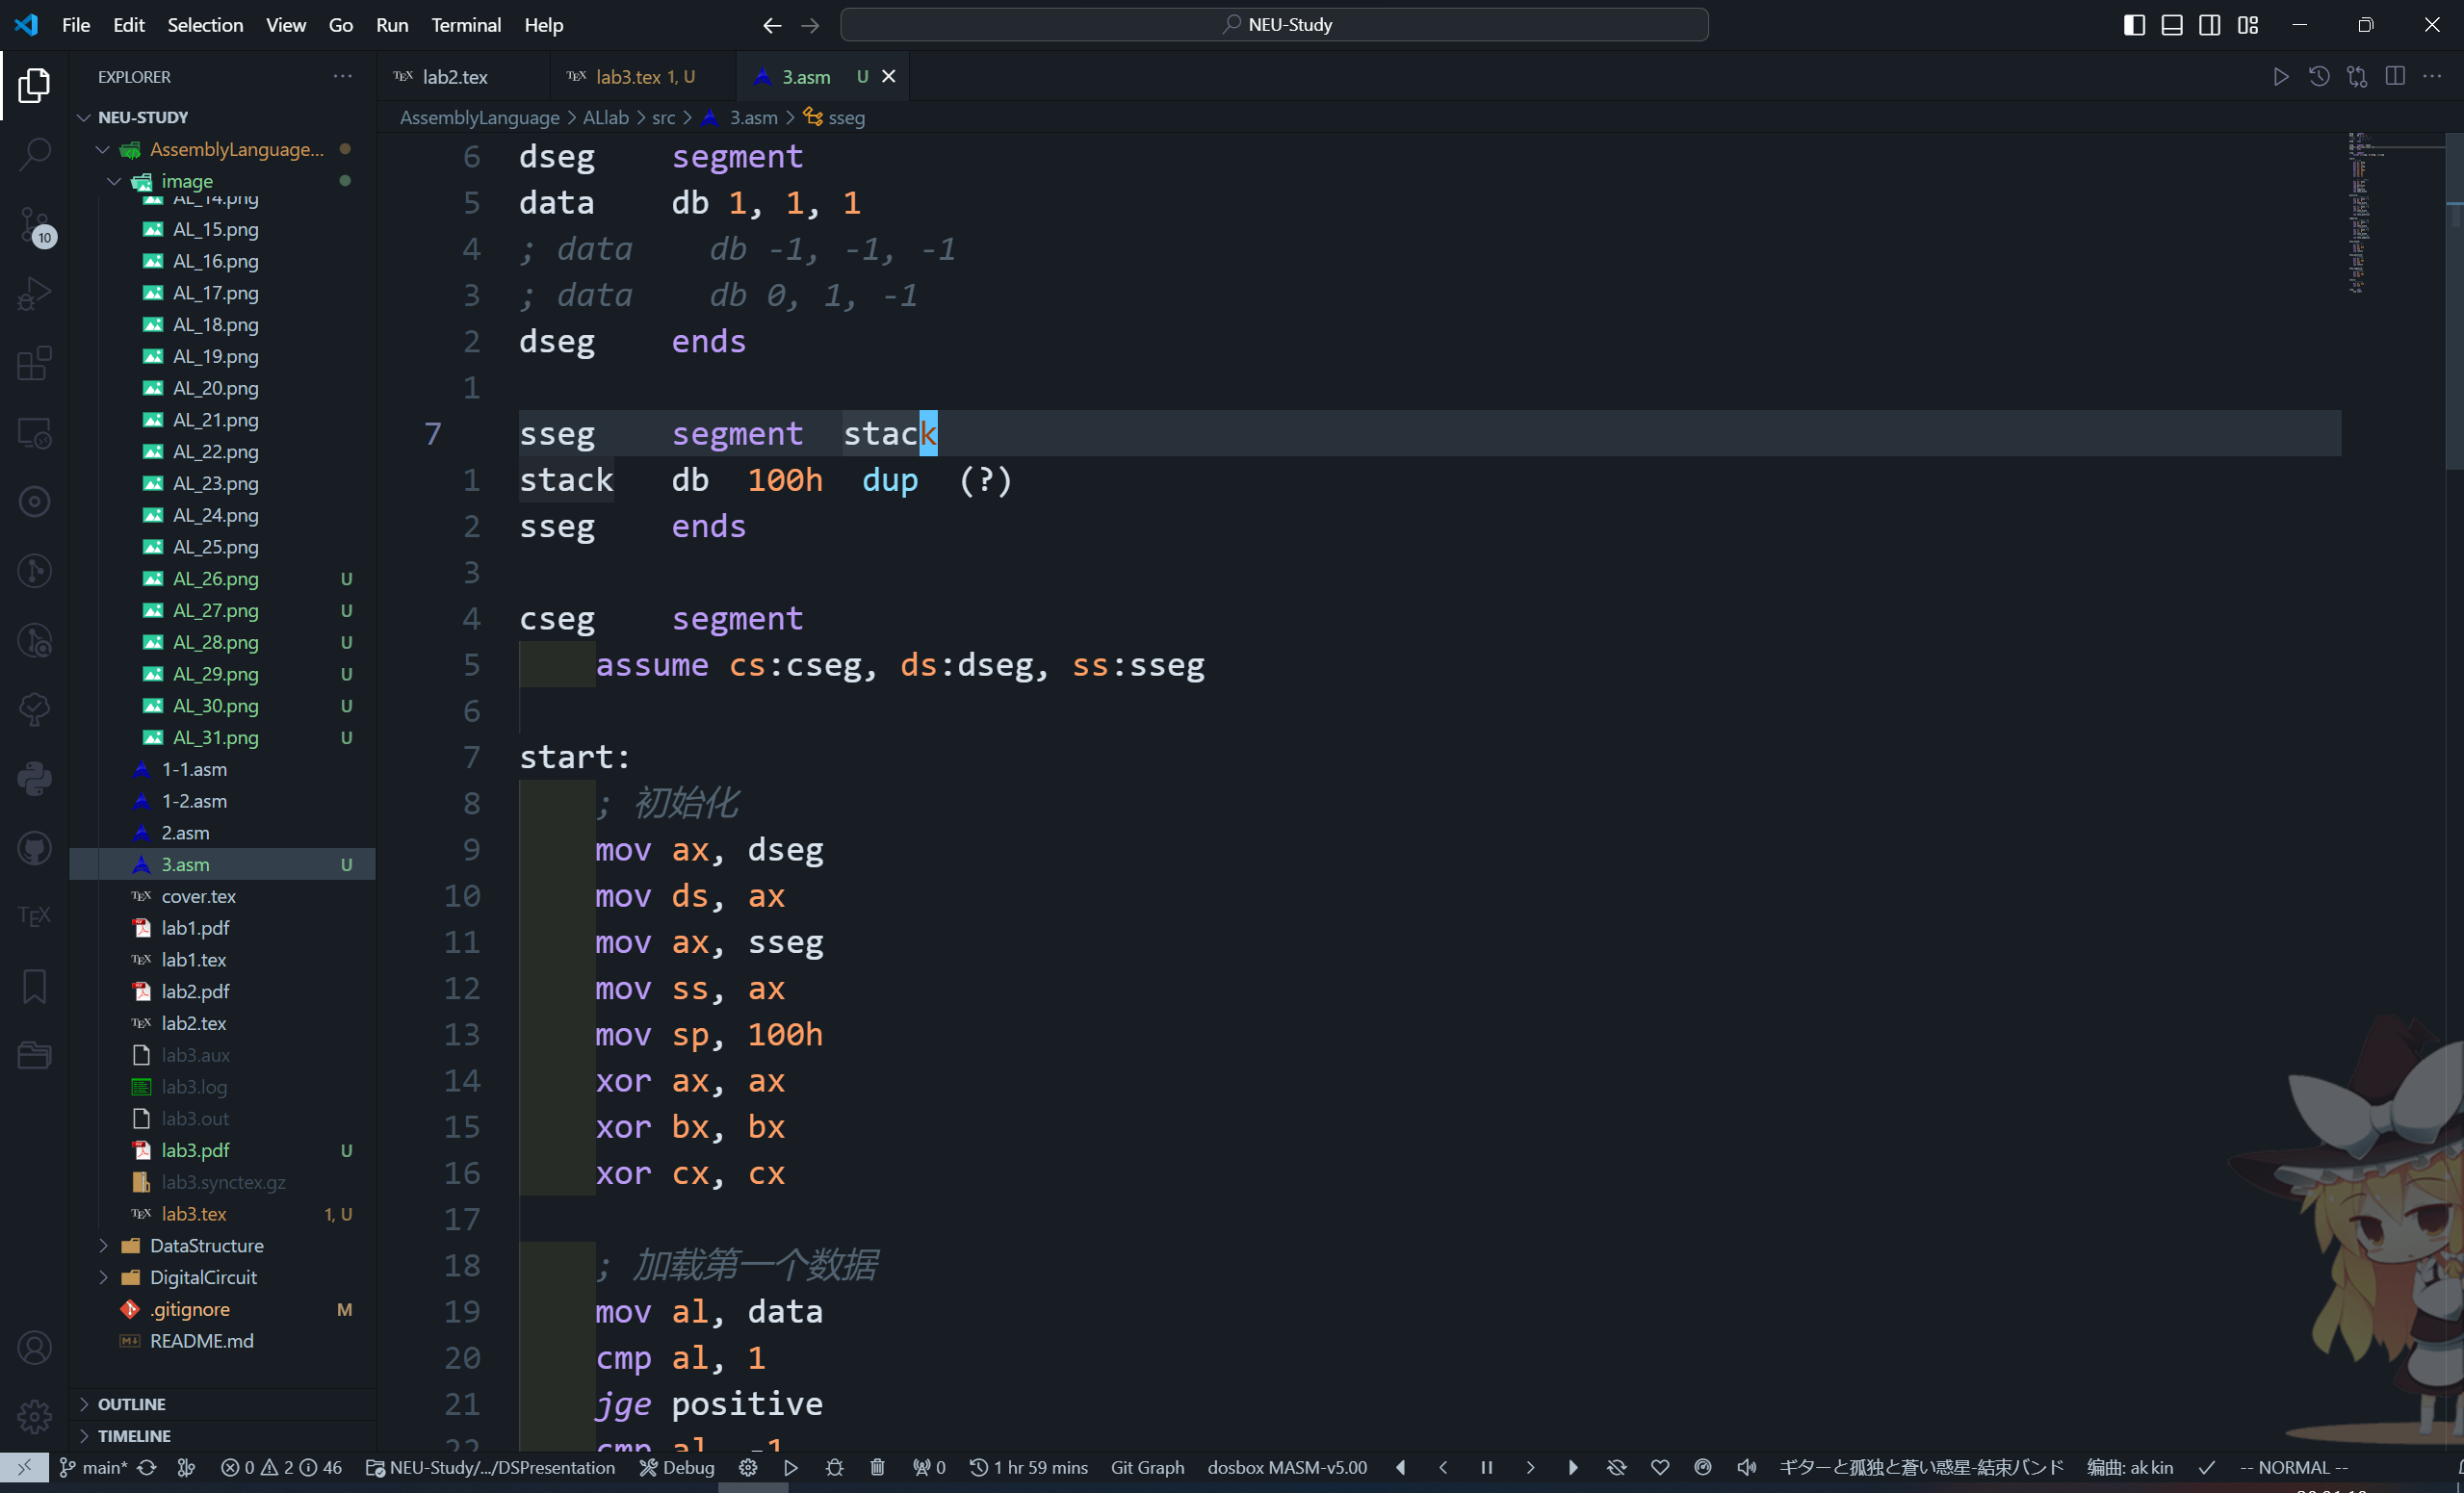
\includegraphics[width=1\textwidth]{image/AL_35.png}\end{center}
    修改数据为0：
    \begin{center}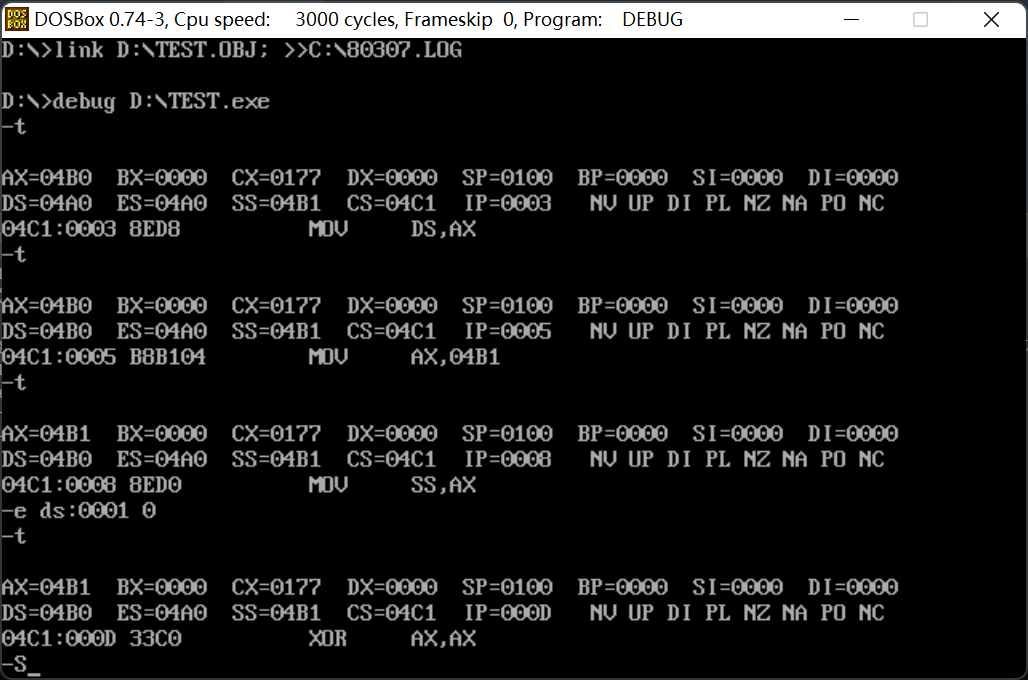
\includegraphics[width=1\textwidth]{image/AL_36.png}\end{center}
    输出空格：
    \begin{center}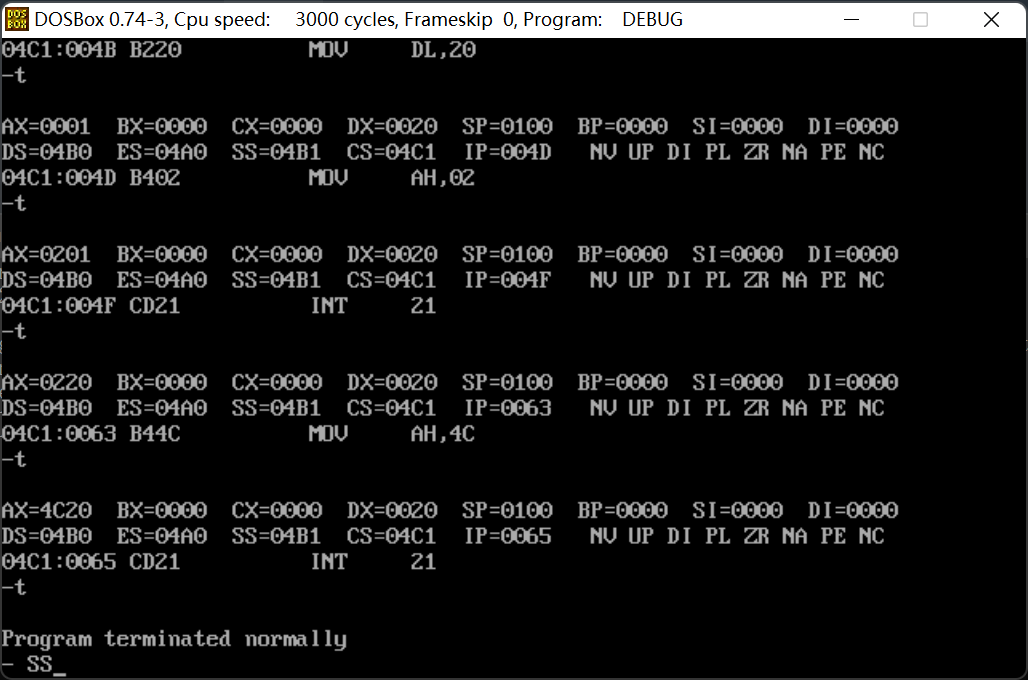
\includegraphics[width=1\textwidth]{image/AL_37.png}\end{center}
    \subsection{流程图}
    \begin{center}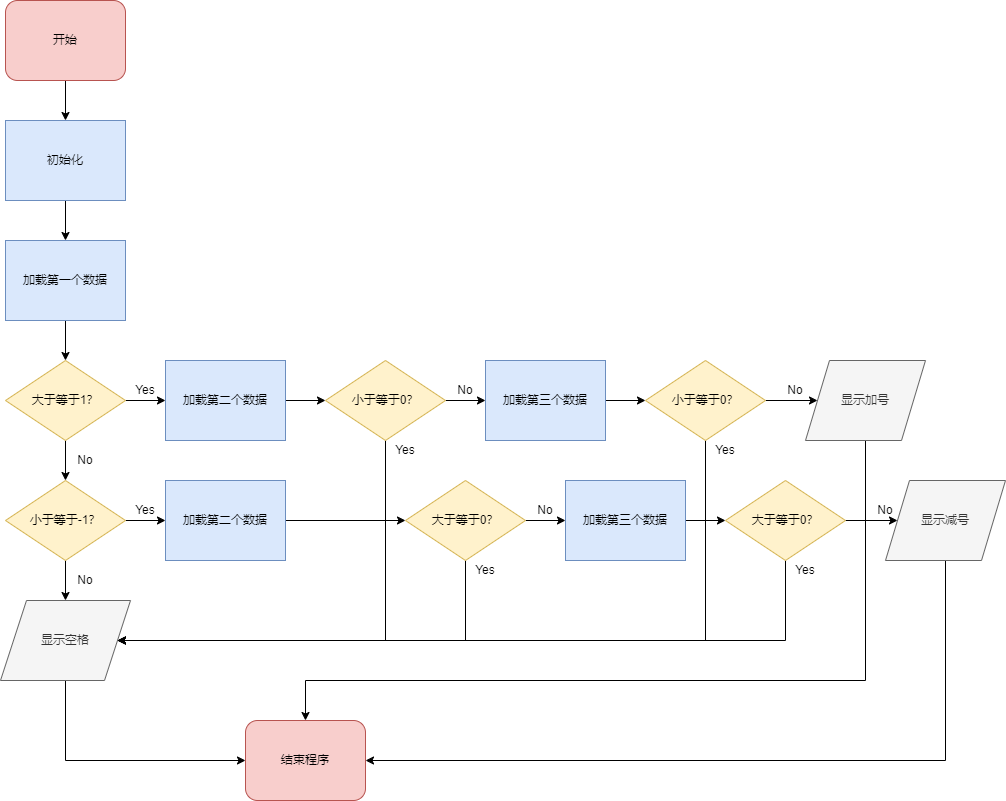
\includegraphics[width=1\textwidth]{image/AL_38.png}\end{center}

\section{心得体会}

通过本次实验，我深入了解并实践了汇编语言，特别是在条件判断和系统调用方面的应用。
此外，我也对程序控制流的复杂逻辑有了更加深刻的认识。

\begin{flushright}\begin{tabular}{rl}
    姓名: & 李俊洁\\
    班级: & 计算机2204 \\
    学号: & 20225443 \\
    课程: & 汇编语言程序设计 \\
    日期: & April 10, 2024 \\
    制作: & \LaTeX \\
    & 感谢您的批阅！
\end{tabular}\end{flushright}
\end{document}